En este capítulo se presentarán los detalles de diseño del proyecto, basándonos
en el análisis mostrado en el capítulo anterior. El modelo de clases de diseño
representado aquí es más fiel a la implementación final que el diagrama de
clases conceptuales, pero aún así hay detalles que no se han contemplado por ser
demasiado cercanos a los detalles de implementación.

También en el presente capítulo se detallarán las decisiones de diseño en
relación al aspecto visual de la aplicación, extendiéndonos en el proceso de
creación del logotipo del juego así como de la interfaz gráfica de usuario.

\section{Diagrama de clases de diseño}

Tras la fase de diseño, componían el sistema más de 40 clases, por lo que hemos
tenido que dividir los diagramas en varias partes, intentando seguir cierto
criterio a la hora de elegir qué clases formarán parte de cada división.

En todos los diagramas aparecen, en aras de mantener el contexto, las clases
básicas de la aplicación: \textit{Juego} y \textit{Estado}. Además, hay algunas
otras clases que también se repetirán entre diagramas por conveniencia.

\begin{itemize}
\item En el primer diagrama (figura~\ref{diagrama_clases_1}) aparecen las clases
  relacionadas con el \textit{menú principal}, clases de utilidades (logging y
  animación), y clases para representar elementos gráficos.
\item En el segundo diagrama (figura~\ref{diagrama_clases_2}) aparecen las
  clases relacionadas con el subsistema de análisis del audio, así como las
  secciones \textit{Analizador de Notas} y \textit{Calibrar micrófono}.
\item En el tercer diagrama (figura~\ref{diagrama_clases_2}) aparecen todas las
  clases relacionadas con la sección de \textit{Canciones}.
\item En el cuarto y último diagrama (figura~\ref{diagrama_clases_2}) aparecen
  las clases relacionadas con el motor de \textit{lecciones}.
\end{itemize}

\begin{figure}[htp!]
  \centering
  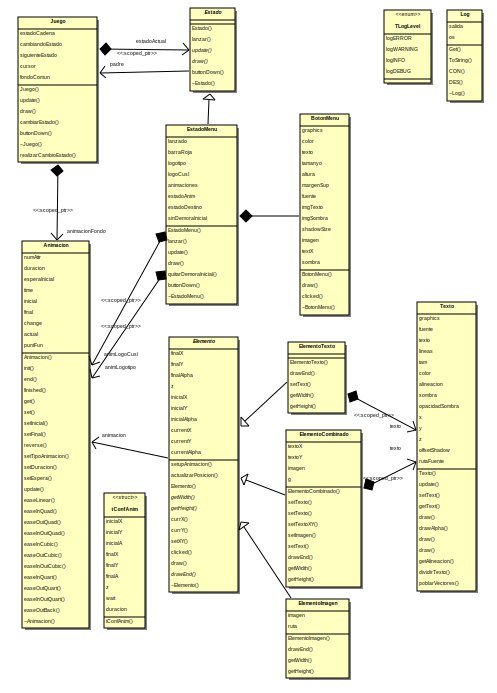
\includegraphics[width=\textwidth]{5_diseno/diagrama1}
  \caption{Diagrama de clases de diseño, parte I}
  \label{fig:diagrama_clases_1}
\end{figure}

\begin{figure}[htp!]
  \centering
  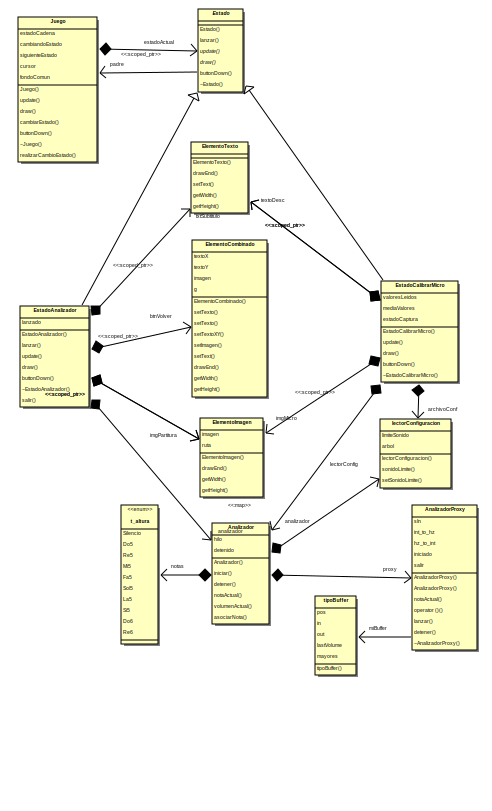
\includegraphics[width=\textwidth, clip=true, trim=0cm 3.5cm 0cm 0cm]{5_diseno/diagrama2}
  \caption{Diagrama de clases de diseño, parte II}
  \label{fig:diagrama_clases_2}
\end{figure}

\begin{figure}[htp!]
  \centering
  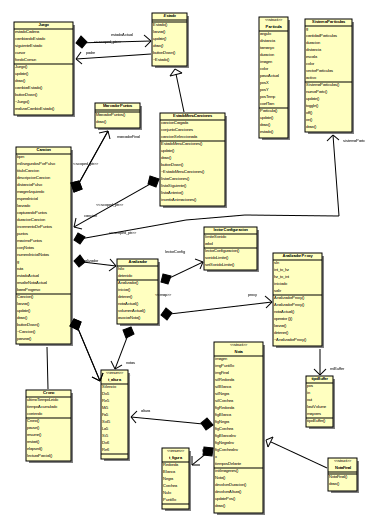
\includegraphics[width=\textwidth, clip=true, trim=0cm 0cm 0cm 0cm]{5_diseno/diagrama3}
  \caption{Diagrama de clases de diseño, parte III}
  \label{fig:diagrama_clases_3}
\end{figure}

\begin{figure}[htp!]
  \centering
  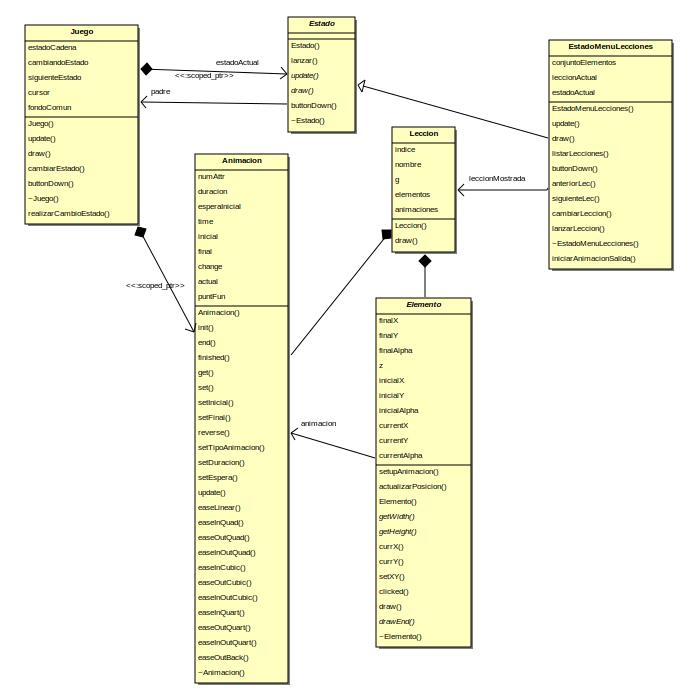
\includegraphics[width=\textwidth, clip=true, trim=0cm 0cm 0cm 0cm]{5_diseno/diagrama4}
  \caption{Diagrama de clases de diseño, parte IV}
  \label{fig:diagrama_clases_4}
\end{figure}

%%% Local Variables: 
%%% mode: latex
%%% TeX-master: "../memoria"
%%% End: 
